\documentclass[border=10pt,tikz]{standalone}

\usepackage{amsmath}
\usepackage{xcolor}
\usepackage{tikz}
\usetikzlibrary{arrows.meta,calc,positioning}

\definecolor{seBlue}{HTML}{2B6CB0}
\definecolor{sePurple}{HTML}{6B46C1}
\definecolor{seGreen}{HTML}{2F855A}
\definecolor{seOrange}{HTML}{D55E00}
\definecolor{seRed}{HTML}{B8323C}
\definecolor{seInk}{HTML}{243B53}
\definecolor{seMuted}{HTML}{52667A}

\begin{document}

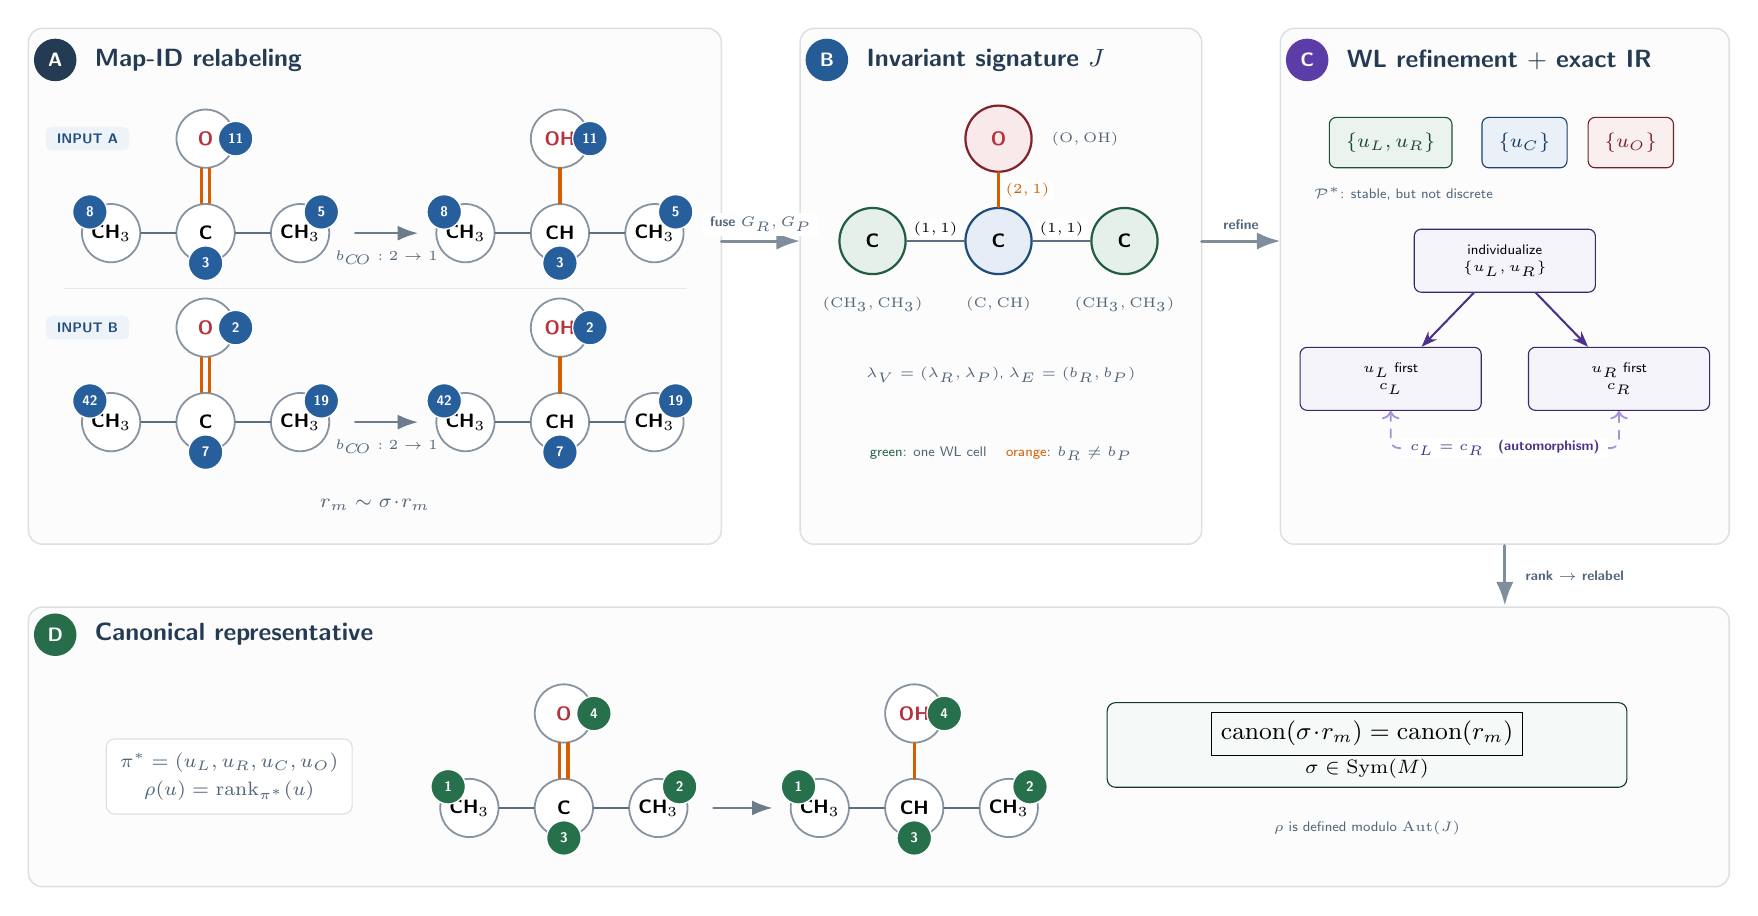
\begin{tikzpicture}[
  x=1cm,
  y=1cm,
  font=\sffamily,
  line cap=round,
  line join=round,
  panel/.style={
    rounded corners=5pt,
    draw=seInk!16,
    fill=seInk!1.5,
    line width=0.55pt
  },
  paneltitle/.style={
    anchor=west,
    font=\sffamily\small\bfseries,
    text=seInk
  },
  panelsubtitle/.style={
    anchor=west,
    font=\sffamily\scriptsize,
    text=seMuted
  },
  letter/.style={
    circle,
    minimum size=5.4mm,
    inner sep=0pt,
    fill=seInk,
    text=white,
    font=\sffamily\scriptsize\bfseries
  },
  chip/.style={
    rounded corners=2pt,
    fill=seBlue!8,
    text=seBlue!72!black,
    font=\sffamily\tiny\bfseries,
    inner xsep=4pt,
    inner ysep=2.5pt
  },
  atom/.style={
    circle,
    minimum size=7.4mm,
    inner sep=0pt,
    draw=seInk!55,
    fill=white,
    line width=0.65pt,
    font=\sffamily\scriptsize\bfseries
  },
  jointatom/.style={
    circle,
    minimum size=8.4mm,
    inner sep=0pt,
    fill=white,
    line width=0.8pt,
    font=\sffamily\scriptsize\bfseries
  },
  mapbadge/.style={
    circle,
    minimum size=4.4mm,
    inner sep=0.25pt,
    draw=white,
    line width=0.5pt,
    fill=seBlue!88!black,
    text=white,
    font=\sffamily\tiny\bfseries
  },
  canonbadge/.style={
    mapbadge,
    fill=seGreen!84!black
  },
  bond/.style={draw=seInk!74, line width=0.9pt},
  changedbond/.style={draw=seOrange, line width=1.2pt},
  edgelabel/.style={
    font=\sffamily\tiny,
    fill=white,
    inner xsep=1.5pt,
    inner ysep=1pt
  },
  atomcaption/.style={font=\sffamily\tiny,text=seMuted},
  note/.style={font=\sffamily\tiny,text=seMuted,align=center},
  reactionarrow/.style={
    -{Latex[length=2.6mm,width=1.9mm]},
    draw=seInk!67,
    line width=0.85pt
  },
  flow/.style={
    -{Latex[length=3.0mm,width=2.2mm]},
    draw=seInk!58,
    line width=1.1pt
  },
  flowlabel/.style={
    fill=white,
    inner xsep=2.5pt,
    inner ysep=1.5pt,
    font=\sffamily\tiny\bfseries,
    text=seMuted
  },
  cell/.style={
    rounded corners=2.5pt,
    minimum height=6.4mm,
    inner xsep=6pt,
    font=\sffamily\scriptsize\bfseries
  },
  tree/.style={
    -{Stealth[length=2.0mm,width=1.5mm]},
    draw=sePurple!72!black,
    line width=0.75pt
  },
  treenode/.style={
    rounded corners=2.5pt,
    draw=sePurple!55!black,
    fill=sePurple!6,
    minimum width=2.3cm,
    minimum height=8mm,
    align=center,
    font=\sffamily\tiny
  },
  infobox/.style={
    rounded corners=3pt,
    draw=seInk!16,
    fill=white,
    font=\sffamily\tiny,
    text=seMuted,
    align=center,
    inner sep=5pt
  },
  invariant/.style={
    rounded corners=3pt,
    draw=seGreen!44!black,
    fill=seGreen!5,
    minimum height=9.5mm,
    align=center,
    font=\sffamily\small
  }
]

% ==========================================================================
% Panel A -- two differently numbered versions of one mapped reaction
% ==========================================================================

\draw[panel] (0,0) rectangle (8.80,6.55);
\node[letter] at (0.34,6.15) {A};
\node[paneltitle] at (0.72,6.15) {Map-ID relabeling};

% ---- input A ----
\node[chip] at (0.75,5.15) {INPUT A};

\node[atom] (aRL) at (1.05,3.95) {CH$_3$};
\node[atom] (aRC) at (2.25,3.95) {C};
\node[atom] (aRR) at (3.45,3.95) {CH$_3$};
\node[atom,text=seRed] (aRO) at (2.25,5.15) {O};
\draw[bond] (aRL)--(aRC);
\draw[bond] (aRC)--(aRR);
\draw[changedbond,transform canvas={xshift=-1.5pt}] (aRC)--(aRO);
\draw[changedbond,transform canvas={xshift=1.5pt}] (aRC)--(aRO);
\node[mapbadge] at (aRL.135) {8};
\node[mapbadge] at (aRC.270) {3};
\node[mapbadge] at (aRR.45)  {5};
\node[mapbadge] at (aRO.0)   {11};

\draw[reactionarrow] (4.15,3.95)--(4.95,3.95);
\node[atomcaption] at (4.55,3.64) {\(b_{C\!O}:2\to1\)};

\node[atom] (aPL) at (5.55,3.95) {CH$_3$};
\node[atom] (aPC) at (6.75,3.95) {CH};
\node[atom] (aPR) at (7.95,3.95) {CH$_3$};
\node[atom,text=seRed] (aPO) at (6.75,5.15) {OH};
\draw[bond] (aPL)--(aPC);
\draw[bond] (aPC)--(aPR);
\draw[changedbond] (aPC)--(aPO);
\node[mapbadge] at (aPL.135) {8};
\node[mapbadge] at (aPC.270) {3};
\node[mapbadge] at (aPR.45)  {5};
\node[mapbadge] at (aPO.0)   {11};

\draw[seInk!12,line width=0.5pt] (0.45,3.25)--(8.35,3.25);

% ---- input B ----
\node[chip] at (0.75,2.75) {INPUT B};

\node[atom] (bRL) at (1.05,1.55) {CH$_3$};
\node[atom] (bRC) at (2.25,1.55) {C};
\node[atom] (bRR) at (3.45,1.55) {CH$_3$};
\node[atom,text=seRed] (bRO) at (2.25,2.75) {O};
\draw[bond] (bRL)--(bRC);
\draw[bond] (bRC)--(bRR);
\draw[changedbond,transform canvas={xshift=-1.5pt}] (bRC)--(bRO);
\draw[changedbond,transform canvas={xshift=1.5pt}] (bRC)--(bRO);
\node[mapbadge] at (bRL.135) {42};
\node[mapbadge] at (bRC.270) {7};
\node[mapbadge] at (bRR.45)  {19};
\node[mapbadge] at (bRO.0)   {2};

\draw[reactionarrow] (4.15,1.55)--(4.95,1.55);
\node[atomcaption] at (4.55,1.24) {\(b_{C\!O}:2\to1\)};

\node[atom] (bPL) at (5.55,1.55) {CH$_3$};
\node[atom] (bPC) at (6.75,1.55) {CH};
\node[atom] (bPR) at (7.95,1.55) {CH$_3$};
\node[atom,text=seRed] (bPO) at (6.75,2.75) {OH};
\draw[bond] (bPL)--(bPC);
\draw[bond] (bPC)--(bPR);
\draw[changedbond] (bPC)--(bPO);
\node[mapbadge] at (bPL.135) {42};
\node[mapbadge] at (bPC.270) {7};
\node[mapbadge] at (bPR.45)  {19};
\node[mapbadge] at (bPO.0)   {2};

\node[font=\sffamily\scriptsize,text=seMuted] at (4.40,0.50)
  {\(r_m\sim\sigma\!\cdot\!r_m\)};

% ==========================================================================
% Panel B -- the two-sided signature graph
% ==========================================================================

\draw[panel] (9.80,0) rectangle (14.90,6.55);
\node[letter,fill=seBlue!85!black] at (10.14,6.15) {B};
\node[paneltitle] at (10.52,6.15) {Invariant signature \(J\)};

\node[jointatom,draw=seGreen!70!black,fill=seGreen!12] (jL) at (10.72,3.85) {C};
\node[jointatom,draw=seBlue!70!black,fill=seBlue!12]   (jC) at (12.32,3.85) {C};
\node[jointatom,draw=seGreen!70!black,fill=seGreen!12] (jR) at (13.92,3.85) {C};
\node[jointatom,draw=seRed!70!black,fill=seRed!10,text=seRed] (jO) at (12.32,5.15) {O};

\draw[bond] (jL)--node[edgelabel,above=0.5pt] {\((1,1)\)} (jC);
\draw[bond] (jC)--node[edgelabel,above=0.5pt] {\((1,1)\)} (jR);
\draw[changedbond] (jC)--node[edgelabel,right=0.5pt,text=seOrange,font=\sffamily\tiny\bfseries] {\((2,1)\)} (jO);

\node[atomcaption] at (10.72,3.05) {\((\mathrm{CH_3},\mathrm{CH_3})\)};
\node[atomcaption] at (12.32,3.05) {\((\mathrm{C},\mathrm{CH})\)};
\node[atomcaption] at (13.92,3.05) {\((\mathrm{CH_3},\mathrm{CH_3})\)};
\node[atomcaption,anchor=west] at (12.87,5.15) {\((\mathrm{O},\mathrm{OH})\)};

\node[note] at (12.35,2.15)
  {\(\lambda_V=(\lambda_R,\lambda_P)\), \(\lambda_E=(b_R,b_P)\)};

\node[note] at (12.35,1.15)
  {\textcolor{seGreen!75!black}{green}: one WL cell \quad
   \textcolor{seOrange}{orange}: \(b_R\ne b_P\)};

% ==========================================================================
% Panel C -- WL cells and the individualization branch
% ==========================================================================

\draw[panel] (15.90,0) rectangle (21.60,6.55);
\node[letter,fill=sePurple!86!black] at (16.24,6.15) {C};
\node[paneltitle] at (16.62,6.15) {WL refinement \(+\) exact IR};

\node[cell,draw=seGreen!62!black,fill=seGreen!10,text=seGreen!55!black]
  at (17.30,5.10) {\(\{u_L,u_R\}\)};
\node[cell,draw=seBlue!62!black,fill=seBlue!10,text=seBlue!55!black]
  at (19.00,5.10) {\(\{u_C\}\)};
\node[cell,draw=seRed!62!black,fill=seRed!8,text=seRed!70!black]
  at (20.35,5.10) {\(\{u_O\}\)};

\node[atomcaption,anchor=west] at (16.20,4.45)
  {\(\mathcal{P}^\ast\): stable, but not discrete};

\node[treenode] (root) at (18.75,3.60)
  {individualize\\\(\{u_L,u_R\}\)};
\node[treenode] (lbr) at (17.30,2.10)
  {\(u_L\) first\\\(c_L\)};
\node[treenode] (rbr) at (20.20,2.10)
  {\(u_R\) first\\\(c_R\)};
\draw[tree] (root)--(lbr);
\draw[tree] (root)--(rbr);

\draw[<->,dashed,draw=sePurple!60,line width=0.65pt,rounded corners=3pt]
  (lbr.south) -- (17.30,1.22) -- (20.20,1.22) -- (rbr.south);
\node[font=\sffamily\tiny\bfseries,text=sePurple!72!black,
      fill=white,inner xsep=3pt,inner ysep=1pt] at (18.75,1.22)
  {\(c_L=c_R\) \; (automorphism)};

% ==========================================================================
% Panel D -- a single shared canonical output
% ==========================================================================

\draw[panel] (0,-4.35) rectangle (21.60,-0.80);
\node[letter,fill=seGreen!82!black] at (0.34,-1.15) {D};
\node[paneltitle] at (0.72,-1.15)
  {Canonical representative};

\node[infobox,font=\sffamily\scriptsize] at (2.55,-2.95)
  {\(\pi^\ast=(u_L,u_R,u_C,u_O)\)\\[2pt]
   \(\rho(u)=\operatorname{rank}_{\pi^\ast}(u)\)};

\node[atom] (cRL) at (5.60,-3.35) {CH$_3$};
\node[atom] (cRC) at (6.80,-3.35) {C};
\node[atom] (cRR) at (8.00,-3.35) {CH$_3$};
\node[atom,text=seRed] (cRO) at (6.80,-2.15) {O};
\draw[bond] (cRL)--(cRC);
\draw[bond] (cRC)--(cRR);
\draw[changedbond,transform canvas={xshift=-1.5pt}] (cRC)--(cRO);
\draw[changedbond,transform canvas={xshift=1.5pt}] (cRC)--(cRO);
\node[canonbadge] at (cRL.135) {1};
\node[canonbadge] at (cRC.270) {3};
\node[canonbadge] at (cRR.45)  {2};
\node[canonbadge] at (cRO.0)   {4};

\draw[reactionarrow] (8.70,-3.35)--(9.45,-3.35);

\node[atom] (cPL) at (10.05,-3.35) {CH$_3$};
\node[atom] (cPC) at (11.25,-3.35) {CH};
\node[atom] (cPR) at (12.45,-3.35) {CH$_3$};
\node[atom,text=seRed] (cPO) at (11.25,-2.15) {OH};
\draw[bond] (cPL)--(cPC);
\draw[bond] (cPC)--(cPR);
\draw[changedbond] (cPC)--(cPO);
\node[canonbadge] at (cPL.135) {1};
\node[canonbadge] at (cPC.270) {3};
\node[canonbadge] at (cPR.45)  {2};
\node[canonbadge] at (cPO.0)   {4};

\node[invariant,minimum width=6.6cm] at (17.00,-2.55)
  {\(\boxed{\operatorname{canon}(\sigma\!\cdot\! r_m)
  =\operatorname{canon}(r_m)}\)\\[1pt]
   \scriptsize \(\sigma\in\operatorname{Sym}(M)\)};

\node[note] at (17.00,-3.60)
  {\(\rho\) is defined modulo \(\operatorname{Aut}(J)\)};

% ==========================================================================
% Flow between panels
% ==========================================================================

\draw[flow] (8.80,3.85)--(9.80,3.85);
\node[flowlabel] at (9.30,4.06) {fuse \(G_R,G_P\)};

\draw[flow] (14.90,3.85)--(15.90,3.85);
\node[flowlabel] at (15.40,4.06) {refine};

\draw[flow] (18.75,-0.02)--(18.75,-0.78);
\node[flowlabel,anchor=west] at (18.92,-0.40) {rank \(\rightarrow\) relabel};

\end{tikzpicture}

\end{document}
